%% LyX 2.1.0 created this file.  For more info, see http://www.lyx.org/.
%% Do not edit unless you really know what you are doing.
\documentclass[english,paper=a4,fontsize=10pt]{scrartcl}
\usepackage[T1]{fontenc}
\usepackage[latin9]{inputenc}
\usepackage{color}
\usepackage{babel}
\usepackage{amsthm}
\usepackage{amsmath}
\usepackage{amssymb}
\usepackage{esint}
\usepackage[numbers]{natbib}
\usepackage[unicode=true,
 bookmarks=true,bookmarksnumbered=true,bookmarksopen=false,
 breaklinks=false,pdfborder={0 0 0},backref=false,colorlinks=true]
 {hyperref}
\hypersetup{
 urlcolor=webbrown,linkcolor=Blue,citecolor=webgreen}

\makeatletter
%%%%%%%%%%%%%%%%%%%%%%%%%%%%%% Textclass specific LaTeX commands.
\RequirePackage{todonotes}
\theoremstyle{plain}
\newtheorem{thm}{\protect\theoremname}
  \theoremstyle{definition}
  \newtheorem{defn}[thm]{\protect\definitionname}

%%%%%%%%%%%%%%%%%%%%%%%%%%%%%% User specified LaTeX commands.
% article example for classicthesis.sty
 % KOMA-Script article 
\usepackage[nochapters]{classicthesis}% nochapters
\let\oldtitle\title
\renewcommand{\title}[1]{\oldtitle{\rmfamily\normalfont\spacedallcaps{#1}}}
\let\oldauthor\author
\renewcommand{\author}[1]{\oldauthor{\spacedlowsmallcaps{#1}}}
\date{}

\definecolor{Blue}{cmyk}{1, 0.878, 0, 0}
\usepackage{tikz}
\usepackage{pgfplots}
\usepackage{amssymb}

\makeatother

  \providecommand{\definitionname}{Definition}
\providecommand{\theoremname}{Theorem}

\begin{document}

\title{Physician Information Acquisition In a Dynamic Setting}


\author{Rud Faden}

\maketitle
\tableofcontents{}


\section{The Patient}

Following \citep{Rochaix1989}, the patient has a utility function
\begin{eqnarray*}
U & = & u(t,s)
\end{eqnarray*}


where $t$ is treatment, $s$ is disease variable classified by its
severity of illness, which belongs to an interval $[a,b]$, where
$a$ is the minimum level of severity and $b$ is the maximum. The
patient has a preference over the level of treatment $t\in\mathbb{R}^{+}$,
where $t$ is a mix of inputs used. $U$ is a von Neumann--Morgenstern
utility function, which is three times differential. It is also assumed
that $U$ has both increasing and decreasing segments to capture the
negative health effects of over-treatment. I also assume that increasing
the level of severity, has a negative first derivative $U_{s}<0$,
and that a increase in severity increases the marginal utility of
treatment $(U_{ts}>0)$. Under perfect agency and full information
the maximization problem is simply given by 
\begin{equation}
\max_{t}u(t,s)\ F.O.C\ u_{t}=0\label{eq:eq:full-information}
\end{equation}


for all $s$, there is a unique solution $t^{*}$ to the problem in
\eqref{eq:eq:full-information}, and the variable $t^{*}(s)$ has
a positive first derivative whit respect to $s$ $(\partial t^{*}/\partial s>0)$
.

\begin{figure}
\resizebox{0.45\textwidth}{!}{%
    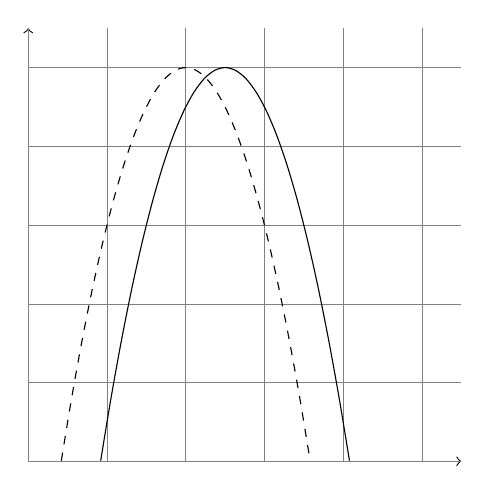
\begin{tikzpicture}
\draw[<->] (0,5.5) -- (0,0)--(5.5,0);
\draw[very thin, color=gray] (0,0) grid (5.5,5.5);
\draw[scale=0.5,domain=0.84:7.16,smooth,variable=\x,dashed] plot ({\x},{10-pow((\x-4),2)});
\draw[scale=0.5,domain=1.84:8.16,smooth,variable=\x] plot ({\x},{10-pow((\x-5),2)});
    \end{tikzpicture}
}

\protect\caption{The patients utility functions}


\end{figure}



\subsection{Uncertainty with perfect agency}

In reality however, $s$ is never observed. The level of severity
for the patients a random variable represented by $S$, characterized
by a subjective density function $f(s,\theta)$, where $s$ is a realization
of $S$ with support in $[a,b]$ and $\theta$ is a parameter that
describes the uncertainty about $s$. Higher $\theta$'s corresponds
to more uncertainty about $s$.%
\footnote{In the extreme case where the agent has no clue about $s$, $\theta$
is a uniform distribution%
} The expected value of choosing an admissible treatment intensity$t$
is given by 
\begin{equation}
u(t,\theta)=E[u(t,s)]=\max_{t}\int_{a}^{b}u(t,s)f(s,\theta)ds\label{eq:expected-utility-prior}
\end{equation}


It is however possible to acquire costly information about $s$ through
medical diagnostics and physician effort. However, for information
to be a desirable good we must have that more information makes the
patient better off. As it it not possible to know the result of the
information before it is obtained it is not exactly clear that more
information is always better than less. For example, a ``surprising''
observation will increase, rather than decrease, the uncertainty about
$d$. Therefore we need a way to order information. Assume that for
each $\gamma\in[0,\infty]$ there is a potentially observable random
variable $\tilde{x}_{\gamma}$ which is correlated with $d$ such
that for $\gamma<\gamma'$ $\tilde{x}$ is sufficient for $\tilde{x}'$
as defined by \citep{Blackwell1953}. Then it is possible to interpret
$\gamma$ as a measure of the amount of information conveyed by $\tilde{x}$,
such that smaller $\gamma$'s indicate more informative. 
\begin{defn}
\label{def:sufficiency}Let $f(x\mid d,\gamma)$ be the likelihood
function. An observation of the random variable $\tilde{x}$ is sufficient
for all observation of the random variable $\tilde{x}'$ if there
exists a conditional density function $g$ such that 
\[
f(x_{\gamma},d,\gamma')=\int_{X}g(x_{\gamma}'\mid x)f(x_{\gamma}\mid d,\gamma)dx_{\gamma}\,\forall x_{\gamma},d
\]


where $X$ is the sample space of $\tilde{x}$. \citep{Kihlstrom1974a}
\end{defn}
After observing $x$, the physician updates his prior by Bayes rule
\begin{equation}
f(s\mid x,\gamma)=f(x\mid s,\gamma)f(s,\theta)/f(x,\gamma)\label{eq:Bayes}
\end{equation}


The change in the physicians expectation about $d$ from observing
the realization of $\tilde{x}_{\gamma}=x$ change the expected utility.
When $x$ is observed, the expected utility is now given by 
\begin{equation}
u(t,\theta,x)=E[u(t,s,x)]=\max_{t}\int_{a}^{b}u(t,s)f(s\mid x,\gamma)ds\label{eq:updated-bayes}
\end{equation}


however, as the physician does not a priori know what information
he receives from $\tilde{x}_{\gamma}$, we must average his expectation
in \ref{eq:updated-bayes} by the probability of all realization of
$\tilde{x}_{\gamma}.$ Therefore the decision about the amount of
treatment $t$ is based on the maximization of 
\begin{equation}
u(t,\theta,\gamma)=E[u(t,s,x)]=\int_{X}\max_{t}\left\{ \int_{a}^{b}u(t,s)f(s\mid x,\gamma)ds\right\} f(x,\gamma)dx\label{eq:expected-update}
\end{equation}


In equation \ref{eq:expected-update} we might similarly to $\theta$
interpret the parameter $\gamma$ to measure the degree of uncertainty
about the information received. If the sufficiency condition holds,
such that for $\gamma<\gamma'$ the information generated by $\tilde{x'}_{\gamma}$
is a garbling of $\tilde{x}_{\gamma}$, then \citet[theorem 6.3]{Marschak1968}
has shown that utility increases, as $\gamma$ decreases. 

Medical diagnostics and physician effort is, however, not free. To
capture the cost of information I define the cost function $C(\gamma)$
where $C$ is the price of observing $\tilde{x}_{\gamma}$ in utiles.
It is assumed that $C'(\gamma)>0$ and $C''(\gamma)>0$.

The physician must then make his decision about $t$ about $\gamma$
sequentially. First the physician chooses a quantity of information
$\gamma$ and then chooses a treatment that maximizes expected utility.
However, as information cannot be returned, the physician must base
his decision of $\gamma$ on the maximization of \ref{eq:expected-posterior}
\begin{equation}
u(t,\theta,\gamma)=E[u(t,s,x)]=\max_{\gamma}\left[\int_{X}\max_{t}\left\{ \int_{a}^{b}u(t,s)f(s\mid x,\gamma)ds\right\} f(x,\gamma)dx-C(\gamma)\right]\label{eq:expected-posterior}
\end{equation}



\subsubsection{Case 1: a change in severity of illness}

An increase in the severity of illness can be archived by shifting
the patients distribution of $d$ to the right. let $\Delta$ be the
distance by which the distribution is shifted and leave all other
moments of the distribution unchanged. Then let $f(s,\theta)=q(s-\Delta,\theta)$,
so that the distribution of $f$ is simply the distribution of $q$
shifted to the right by the distance $\Delta$ for all $s$.


\subsubsection{Case 2: a change in the riskiness of $d$}


\subsubsection{Case 3: a change in the riskiness of the signal $s$}

\bibliographystyle{plainnat}
\bibliography{C:/Users/okorf/Dropbox/PhD/Bibtexfiles/library}

\end{document}
